\documentclass{ifacconf}
\usepackage{standalone}
\usepackage{times}
\usepackage{float}
\usepackage{amsmath}
\usepackage{graphicx}      % include this line if your document contains figures
\usepackage{natbib}        % required for bibliography
%===========================================
%% Additional packages
\usepackage{times}
\usepackage{amsmath}
\usepackage{amsthm}
\usepackage{amssymb}
\usepackage{amsfonts}
\usepackage{mathtools}
%\usepackage{calc}
\usepackage{subfigure}
\usepackage{graphicx}
\usepackage{color}
\usepackage{url}
%\usepackage{lineno}
%\usepackage{ulem} % for underlining and strike through
%\normalem % reset emph to normal
%\usepackage{setspace} % for line spacing - e.g. 1.5, 2
\usepackage[usenames,x11names]{xcolor}
%\usepackage{xspace} % for inserting a space in TeX commands if needed
%\usepackage{caption}
\usepackage[bookmarks=true]{hyperref}
%\renewcommand{\thesubfigure}{\relax} % no subfig counters
%\let\chapter\section % algorithm2e natbib compatibility
%\usepackage{accents}
%\usepackage[titletoc,toc,title]{appendix}
%\usepackage{longtable}
%\usepackage{setspace}
\usepackage{multicol}

%% Packages
%\usepackage[margin=1in]{geometry}
%\usepackage[abs]{overpic}
\usepackage[linesnumbered,vlined,ruled]{algorithm2e}
%\usepackage{multirow} % for cell tables spanning multiple rows
\usepackage{tikz,pgf}%,tikz-3dplot}
\usetikzlibrary{arrows,automata,shapes,calc,backgrounds,spy,positioning}
%\usetikzlibrary{external}
%\tikzexternalize
%\usepackage[numbers]{natbib}
%\usepackage[sort,round]{natbib}
%\usepackage{lipsum}
\usepackage{epstopdf}

\theoremstyle{plain}
\newtheorem{theorem}{Theorem}
\newtheorem{cor}{Corollary}
\newtheorem{prop}{Proposition}
\newtheorem{lemma}{Lemma}

\theoremstyle{definition}
%\newtheorem{definition}{Definition}
\newtheorem{remark}{Remark}
\newtheorem{cond}{Condition}

\newtheorem{example}{Example}
\newtheorem{problem}{Problem}
%\newtheorem{assumption}{Assumption}


%%% figure path
\graphicspath{{figures/}}

%% Remove footnote mark
%\renewcommand{\footnotemark}{}

%%% Redefine qed symbol
%\renewcommand{\qedsymbol}{$\blacksquare$}

%% Projection symbol
%\newcommand{\project}[1]{\! \upharpoonright_{#1}}


%% Theorems 
%\newtheorem{theorem}{Theorem}[section]
%\newtheorem{proposition}[theorem]{Proposition}
%\newtheorem{corollary}[theorem]{Corollary}
\newtheorem{definition}[theorem]{Definition}
%\newtheorem{lemma}[theorem]{Lemma}
%\newtheorem{remark}[theorem]{Remark}
%\newtheorem{remarks}[theorem]{Remarks}
%\newtheorem{example}[theorem]{Example}
%\newtheorem{algo}[theorem]{Algorithm}
%\newtheorem{problem}[theorem]{Problem}
%\newtheorem{Procedure}[theorem]{Procedure}
%\newcommand{\exampler}[2]{\medskip \hskip -\parindent {\bf Example #1 Revisited.~}{\it #2}\medskip}

%% Percent
%\newcommand\oprocendsymbol{\hbox{$\square$}}
%\newcommand\oprocend{\relax\ifmmode\else\unskip\hfill\fi\oprocendsymbol}
%\def\eqoprocend{\tag*{$\bullet$}}

%% Enumerate environment
%\renewcommand{\labelenumi}{(\roman{enumi})}
%\renewcommand{\labelenumii}{(\alph{enumii})}

%% Breakable comma
%\mathchardef\breakingcomma\mathcode`\,
%{\catcode`,=\active
%  \gdef,{\breakingcomma\discretionary{}{}{}}
%}
%\newcommand{\breqn}[1]{\mathcode`\,=\string"8000 #1}

%% Other Stuff
%\newcommand{\margin}[1]{\marginpar{\tiny\color{blue} #1}}
%%\addtolength{\marginparwidth}{-0.3in}
\newcommand{\todo}[1]{\vskip 0.05in \colorbox{yellow}{$\Box$ \ttfamily\bfseries\small#1}\vskip 0.05in}
%\newcommand{\todo}[1]{}
%\newcommand{\vers}{\operatorname{vers}}

%% Roman, calligraphic, boldface, double barred letters
\newcommand{\RM}[1]{\mathrm{#1}}
\newcommand{\CA}[1]{\mathcal{#1}}
\newcommand{\BF}[1]{\mathbf{#1}}
\newcommand{\IT}[1]{\mathit{#1}}
\newcommand{\BB}[1]{\mathbb{#1}}
\newcommand{\TT}[1]{\mathtt{#1}}
\newcommand{\FK}[1]{\mathfrak{#1}}
\newcommand{\BS}[1]{\boldsymbol{#1}}

%%% Temporal logic symbols
\newcommand{\notltl}{\neg}
\newcommand{\andltl}{\wedge}
\newcommand{\orltl}{\vee}
\newcommand{\Next}{\ensuremath{\bigcirc}}
\newcommand{\Always}{\ensuremath{\ \square\ }}
\newcommand{\Event}{\ensuremath{\ \diamondsuit\ }}
\newcommand{\Until}{\ \CA{U}\ }
\newcommand{\Implies}{\Rightarrow}
\newcommand{\Equiv}{\Leftrightarrow}
%\newcommand{\Not}{\lnot}
\newcommand{\True}{\top}
\newcommand{\False}{\perp}
%\def\prop{\TT{data}}
%\def\popt{\pi}
\newcommand{\AP}{AP}
\newcommand{\pred}{\xi}

\newcommand{\Real}{\BB{R}}

%% Abbreviations
%\def\eg{e.g.\xspace}
%\def\Eg{E.g.\xspace}
%\def\ie{i.e.\xspace}
%\def\Ie{I.e.\xspace}
%\def\etc{etc.\xspace}
%\def\vs{vs.\xspace}
%\def\wrt{w.r.t.\xspace}
%\def\etal{et al.\xspace}

%% Exotic words
\newcommand{\buchi}{B\"uchi\ }

%% Symbols of automata
\newcommand{\PA}{\mathcal{P}}
\newcommand{\BA}{\mathcal{B}}
%\newcommand{\FA}{\mathcal{F}}

\newcommand{\TS}{\mathcal{F}}
\newcommand{\LA}{\mathcal{L}}
\newcommand{\KA}{\mathcal{K}}
\newcommand{\MDP}{\mathcal{M}}
\newcommand{\RA}{\mathcal{R}}
\newcommand{\FSA}{\mathcal{A}}

\newcommand{\TSX}{\BB{V}_\TS}
\newcommand{\TSE}{\BB{E}_\TS}
\newcommand{\TSEE}{\BB{E}}

\newcommand{\DTL}{DTL\xspace}


%% Short macros for arrows
\newcommand{\la}{\leftarrow}
\newcommand{\ra}{\rightarrow}
\newcommand{\ras}[1]{\stackrel{#1}{\rightarrow}}
\newcommand{\asgn}{\la}
\newcommand{\proj}[2]{{#1}{\downharpoonright_{#2}}}

\newcommand{\df}{\xspace\RM{d}}

%% Names of the Algorithms
%\newcommand{\optrun}{\textsc{Optimal-Run}\ }
%\newcommand{\exactmultioptrun}{\textsc{Exact-Multi-Robot-Optimal-Run}\ }
%\newcommand{\constR}{\textsc{Construct-Region-Automaton}\ }
%\newcommand{\constT}{\textsc{Construct-Team-TS}\ }
%\newcommand{\syncT}{\textsc{Sync-Team-TS}\ }
%\newcommand{\boundOpt}{\textsc{Bound-Optimality}\ }

% Custom operators
%\DeclareMathOperator*{\argmin}{arg\,min}
\newcommand{\norm}[1]{\left\| {#1} \right\|}
\newcommand{\norminf}[1]{\left\| {#1} \right\|_{\infty}}
\newcommand{\normeucl}[1]{\left\| {#1} \right\|_{2}}
\newcommand{\abs}[1]{\left| {#1} \right|}
\newcommand{\card}[1]{\left| {#1} \right|}
\newcommand{\spow}[1]{2^{#1}}
%\newcommand{\interior}[1]{\accentset{\smash{\raisebox{-0.12ex}{$\scriptstyle\circ$}}}{#1}\rule{0pt}{2.3ex}}
\newcommand{\interior}[1]{\mathring{#1}}
\DeclareMathOperator{\diag}{diag}
\newcommand{\lift}{\upharpoonright}
%
%% Display a grid to help align images
%\beamertemplategridbackground[1cm]
%\usepackage[style=numeric-comp]{biblatex}
\usepackage{cite}


%\documentclass[letterpaper, 11pt, onecolumn]{TemplateFiles/ieeeconf}
%\IEEEoverridecommandlockouts \overrideIEEEmargins 
%\pagestyle{plain}

%\usepackage[ruled,vlined,linesnumbered,boxruled]{algorithm2e}
%\usepackage{mathrsfs}
%\usepackage{graphicx}
%\usepackage{amsfonts}
%\usepackage{amsmath}
%\usepackage{amssymb}
%\usepackage{array}
%\usepackage{flafter}
%\usepackage{tabu}
%\usepackage{cite}
%\usepackage{subfigure}
%\usepackage{verbatim}
%\usepackage{bbm}
%\usepackage[usenames]{color}
%\usepackage[svgnames]{xcolor}

%\usepackage{balance}

%\usepackage{nicefrac}
%\usepackage{psfrag}
%\usepackage{umoline}
%\usepackage{hyperref}
%\usepackage{appendix} %[2009/09/02 v1.2b extra appendix facilities]
%\let\proof\relax
%\let\endproof\relax
%\usepackage{amsthm}	% This is needed for \newtheorem and proof environment.
% \usepackage{natbib} % for citing the papers with auther-year format in parantheses.
%\usepackage[numbers, sort]{natbib}

%\usepackage{etoolbox}

%\providecommand{\citet}[1]{\citeauthor{#1}\,[\citeyear{#1}]}
%\providecommand{\citep}[1]{\cite{#1}}

%\newtheorem{thm}{Theorem}
%\newtheorem{Def}{Definition}
%\newtheorem{Problem}{Problem}
%\newtheorem{Lem}{Lemma}
%\newtheorem{Cor}{Corollary}
%\newtheorem{assumption}{Assumption}
%\newtheorem{proposition}{Proposition}
%\newtheorem{definition}{Definition}
%\newtheorem{property}{Property}
%\newtheorem{Remark}{Remark}
%\newtheorem{exmp}{Example}[section]
%\newenvironment{proof}[1][Proof]{\begin{trivlist}
%\item[\hskip \labelsep {\bfseries #1}]}{\end{trivlist}}

%\newcommand{\TypeOfDoc}{IJRR} % This either can be TR or Conf or IJRR
%\newcommand{\FinalFlag}{No} % This either can be No or Accepted
%\newtoggle{finalpaper}
%\toggletrue{finalpaper}
%\togglefalse{finalpaper}

\graphicspath{{./figs/}}

%\allowdisplaybreaks[1]

%\newcommand{\kXX}[1]{\color{blue} XX #1 XX \color{black}}
%newcommand{\AXX}[1]{\color{purple} XX #1 XX \color{black}}
\newcommand{\aXX}[1]{\color{orange} #1  \color{black}}
\newcommand{\axx}[1]{\aXX{#1}}


\newcommand{\pr}[1]{\textbf{#1:} }

\newcommand{\codeline}[1]{\par{\ttfamily #1 \par}}  % This line is added because sth like this \newcommand{\initeali}{\verb|InitializeEdge|} does not work. For further details please check out this link % http://tex.stackexchange.com/questions/86071/newcommand-for-verbatim
% please do not delete above comments as it can be really confsing


%%%%%%%%%%%%%%%% symbols
\newcommand{\tv}{\varpi} % tube volume (edge tube volume)
\newcommand{\td}{\Gamma} % tube distance (edge tube distance)

%%%%%%%%%%%%%%%%%%%%%%%%%%%%%%%%%%%%%%%%%%%%%%%%%% To reduce pages
%\textfloatsep = 0pt
%\renewcommand{\baselinestretch}{0.96}
%%%%%%%%%%%%%%%%% Make bibs smaller
%\renewcommand{\IEEEbibitemsep}{0pt plus 2pt}
%\makeatletter
%\IEEEtriggercmd{\reset@font\normalfont\footnotesize}
%\makeatother
%\IEEEtriggeratref{1}

%%%%%%%%%%%%%%%%% margins
%\usepackage{geometry}
% \newcommand{\papermargin}{0.97in} % IEEE asks for 0.75 on all pages, but the first page
% %\newgeometry{top=0.75in,bottom=.75in,right=.75in,left=.75in}
% \newgeometry{top=\papermargin,bottom=\papermargin,right=\papermargin,left=\papermargin}
% \newgeometry{top=1.in,bottom=1.in,right=1.in,left=1.in}

\let\labelindent\relax
\usepackage{enumitem}


\newcommand{\red}[1]{{\color{red} #1}}
\newcommand{\X}{{\mathbb{X}}}
\newcommand{\Y}{{\mathbb{Y}}}
\newcommand{\U}{{\mathbb{A}}}
\newcommand{\A}{{\U}}

\newcommand{\Hist}{{\mathsf{H}}}

\newcommand{\InF}{\mathcal{U}_{v}}
\newcommand{\Wt}{\mathbb{W}_{\mathbb{T}}}
\newcommand{\Fpred}{{\mathcal F}}

\newcommand{\M}{{\mathbf{M}}}

\newcommand{\po}{\mathbb{P}}     % Probability of an event
\newcommand{\p}[1]{\po\left(#1\right)}     % Probability of an event
\renewcommand{\P}{P}
\newcommand{\pd}[1]{p\left(#1\right)}     % Probability density of an event

\renewcommand{\S}{\mathbb S}
\newcommand{\borel}[1]{\mathcal{B}\left(#1\right)}


\newcommand{\eps}{\epsilon} \newcommand{\rel}{\mathcal{R}} % numbers option provides compact numerical references in the text. 

\pdfinfo{
   /Author (S.Haesaert et al.)
   /Title  (Formal abstraction of POMDPs for Distribution LTL)
   /CreationDate (D:20101201120000)
   /Subject (Formal abstraction)
   /Keywords (abstraction;POMDP)
}

% Table caption wrangling
\usepackage{etoolbox}
 



\allowdisplaybreaks[1]
\usetikzlibrary{fit}

\begin{document}


\begin{frontmatter}

\title{\huge Formal abstraction of POMDPs for Distribution LTL}
\thanks[footnoteinfo]{Sponsor and financial support acknowledgment
goes here. Paper titles should be written in uppercase and lowercase
letters, not all uppercase.}

\author[cal]{S. Haesaert} 
\author[cal]{Lars Petter P.  Nilsson} 
\author[mit]{ Cristian-Ioan Vasile}
\author[jpl]{Rohan}
\author[jpl]{ Ali Agh}
\author[cal]{Richard Murray}
\author[cal]{Aaron Ames}

\address[cal]{California Institute of Technology, 
   Pasadena, CA 91125 USA (e-mail: \{haesaert,pettni,ames,murray\}@caltech ).}
\address[mit]{Massachusetts Institute of Technology, 
   Cambridge, MA 02139 USA (e-mail:  cvasile@mit.edu)}
\address[jpl]{Jet Propulsion Laboratory, 
   Pasadena, CA 91109 USA (e-mail: rohan.a.thakker@jpl.nasa.gov)} 
\maketitle
\begin{abstract}
Currently this report mainly includes copies of the  original paper on pulled by Cristi on Temporal logics with beliefs for planning problems.  Goal is to first see how the temporal logic specifications can be defined with measurability in mind. Then we will include this in the original paper, before starting continuing with the development of this report. 
\end{abstract}
\begin{keyword}
Five to ten keywords, preferably chosen from the IFAC keyword list.
\end{keyword}

\end{frontmatter}
%%%%%%%%%%%%%%%%%%%%%%%%%%%%%%%%%%%%%%%%%%%%%%%%
%%%%%%%%%%%%%%%%%%%%%%%%%%%%%%%%%%%%%%%%%%%%%%%%
 
\section{Introduction} \label{subsec:intro}
In this work, we use a language for specifying behavior under uncertainty using formal methods. 
Some of the questions to be tackled are as follows:
\begin{description}
	\item[Framework:] Does it make sense to formulate the DLTL on a specific choice of belief space or sufficient statistic? Can we instead first formulate it on the POMDP and then show that it  is equivalent to a problem on a COMDP?
	\item[Technical:]  What are the minimal measurability conditions that are required such that for given a POMDP and its reduced COMDP  the LTL problem is ``well"-defined (measurable).
	\item[Technical:] Beyond well-definedness, do we also keep soundness and completeness?
	\item[Technical:] When are optimal policies non-randomized?
	\item[Simulation relations]  Use $(\epsilon,\delta)$- simulation relation for doing formal abstractions on the COMDP model.
	Show that it can be used for control refinement.
	\item[Interesting:] How does system identification fit into this picture?
	\item[Simulation relations:] Can we quantify an $(\epsilon,\delta)$-simulation relation between the sampling based model and the original COMDP?
	\item[Computation results:] Improve results for the computation of $(\epsilon,\delta)$-simulation relations for LTI systems. Reformulate LMI requirement from S-procedure to requirements over Polytopes. 
	\item[Scalable computations:] Can we  tackle the computations in a modular fashion. Split up requirements for e.g. the helicopter and the rover and show that the combined system still behaves as required.
	 
\end{description}


\subsection{Literature}
This section contains a summary of related literature.

\subsection{Technical math results for POMDPs}
The reduction of Markov decision problems with incomplete information to problems with complete information has been tackled in
\cite{yushkevich_reduction_1976,rhenius_incomplete_1974}, with respect to Borel states and Borel actions.

In \cite{feinberg2016partially} and in \cite{feinberg2014optimality} the optimality conditions for POMDP problems solved via COMDPs are analyzed. 

In \cite{saldi2017finite}, the convergence of solutions of finite abstractions of COMPDs to the optimal solutions of POMDPs is analyzed. 


Most of the work (including the references given above) has been developed for additive cost functions. 


\subsection{POMDP reachability and safety verification}

In \cite{ding2013optimal}, the optimal control of partially observable systems over safety specifications is analyzed. 
In \cite{LESSER20141989}, the analysis of partially observable systems with as objective reachability is analyzed. 


\subsection{Notation}

For the sets $A$ and $B$ a relation $\rel\subset A\times B$ is a subset of the Cartesian product $A\times B$. The relation $\rel$ relates $x\in A$ with $y\in B$ if $(x,y)\in\rel$, which is equivalently written as $x\rel y$.
%We use the following notation for the mappings $\rel(\tilde A):=\{y: x\rel y,\  x\in \tilde A\}$ and $\rel^{-1}(\tilde B):=\{x: x\rel y,\  y\in \tilde B\}$  for $\tilde A\subseteq A$ and $\tilde B\subseteq B$.




    Let $\Sigma$ be a finite set. The cardinality,
    power set, Kleene- and $\omega$-closures
    of $\Sigma$ are denoted by $\card{\Sigma}$,
    $\spow{\Sigma}$, $\Sigma^*$ and $\Sigma^\omega$,
    respectively.    
    Each member of $\Sigma^*$ and $\Sigma^\omega$ is referred to as ``word" or "sequence". 
    
    
    $A \subseteq \BB{R}^n$ and $B \subseteq \BB{R}^m$,
    $n, m \geq 0$, we denote by $\CA{M}(A, B)$ the set of
    functions with domain $A$ and co-domain $B$, where $A$ has positive measure with
    respect to the Lebesgue measure of $\BB{R}^n$.
    
    
    The set of all positive semi-definite matrices of size
    $n \times n$, $n \geq 1$, is denoted by $\S^n$.    The $m \times n$ zero matrix and
    the $n \times n$ identity matrix are denoted by
    $\BF{0}_{m, n}$ and $\BF{I}_n$, respectively.
    The supremum and Euclidean norms are denoted by
    $\norminf{\cdot}$ and $\normeucl{\cdot}$, respectively.
    For a given set $\Y$ a metric or distance function $\mathbf d_\Y$ is a function $\mathbf{d}_\Y: \Y\times \Y\rightarrow \mathbb R_{\ge 0}$ 
satisfying the following conditions: 
$\forall y_1,y_2,y_3\in\Y$:
$\mathbf d_\Y(y_1,y_2)=0$ iff $y_1=y_2$; 
$\mathbf d_\Y(y_1,y_2)=\mathbf d_{\Y}(y_2,y_1)$;  and
$\mathbf d_\Y(y_1,y_3)\leq \mathbf d_\Y(y_1,y_2) +\mathbf d_\Y(y_2,y_3)$. 
 %
For metric space $\mathbb S$, we denote with  $\mathcal{B}(\mathbb S)$ its Borel $\sigma$-field. That is  $\mathcal{B}(\mathbb S)$ is the  
collection of all sets that can be formed from countable unions and intersections of open sets.
We refer to  $(\mathbb S,\mathcal{B}(\mathbb S))$ as a Borel measurable space and we denote with $\mathcal P(\mathbb S)$ the set of probability measures on $(\mathbb S,\mathcal{B}(\mathbb S))$.
Together with the measurable space $(\mathbb S,\mathcal{B}(\mathbb S))$,  a probability measure $\po$ defines the probability space, denoted by $(\X,\mathcal{B}(\mathbb S),\po)$ and has realizations  $s\sim \po$.   
Polish spaces are complete separable metric spaces, c.f. \cite{bogachev2007measure}. 

    $\BB{E}[\cdot]$ is the expectation operator.

    
    
\section{Partially observable Markov decision Processes}
In this section, we  analyze the formulation of distribution temporal logics as originally given in \cite{JonesDTL2013} for POMDPS. 
First, we give the definition of POMDPs. Then,  we  give the definition of distribution temporal logic. 


The reachability problem can be formulated with a multiplicative cost function or by using a terminal cost function. In the latter case, the terminal function 


 

\subsection{POMDP}\label{sec:POMDP}
\begin{definition}[general Markov decision process (gMDP)] \label{def:MDP}
A discrete-time partially observable Markov decision process (POMDP) with Borel spaces
\begin{enumerate}
	\item $\X$, the state space with states $x\in\X$ as its element;
	\item $\U$, the action space;
	\item $\Y$, observation space.
\end{enumerate}
with 
\begin{enumerate}
\item $\mu$ the initial probability distribution
\item $p(\cdot|x,a)$ the transition probability of the next state given the current state-action pair
\item $r(\cdot|x)$ the observation channel giving the probability of the current observation given the current state variable $x$	
\end{enumerate}


\end{definition} 

The control can be designed based on the history of observed outputs. Thus, we defined the history space $\Hist_0=\Y$, and $\Hist_t=(\Y\times \U)^t\times \Y$ for $t=1,2,3,\ldots$ endowed the product Borel algebra generated by $\mathcal B (\Y)$ and $\mathcal B(\U)$.
A policy $\pi$ is a sequence of stochastic kernels on $\U$ given $\Hist_t$. 
We denote with $\Pi$ the set of all policies.



By the theorem of Ionescu Tulcea \cite{hll1996}, there exists a unique probability measure $\P_\pi^\mu$ on the canonical space $\Omega:=\Hist_\infty\times\X^\infty$. Thus for a given policy the POMDP defines a stochastic process on the probability space  
 $(H_\infty\times \X^\infty,\mathcal F,\P_\pi^\mu)$.
% \begin{align*}
%   P_\pi^\mu(x_0\in B) = \pi(B),\quad P_\pi^\rho(u_n\in C|h_n) = \rho_n(C|h_n),\quad P_\pi^\rho(x_{n+1}\in B|h_n,u_n) = \mathbb T(B|x_n,u_n),
% \end{align*}

As a special case of the POMDP, we consider a POMDP represented via difference equations which are subject to process noise and observation noise.
\begin{align*}
x_{k+1}&=f(x_k,u_k,w_k)\\
z_k&=h(x_k,v_k)
\end{align*}
where $w_k\sim p_w(\cdot|x_k)$ and $v_k\sim p_v(\cdot|x_k)$ are independent realizations of the the process noise and the observation noise.


 \subsection{Belief space}
Due to the noisy and partial observation of the state, the best one can infer about the system state at time  $t$ is a probability distribution over its possible states
\begin{align}
	b_t(\cdot)=\P(x_t\in \cdot|\Hist_t )\in \mathcal P (\X)
\end{align}
This state distribution is referred to as the belief state $b_t(\cdot)$. 
The Belief space (i.e., the set of all beliefs) is denoted by $\mathbb{B}\subset \mathcal P(\X)$.
It can be shown that the transitions of this belief state evolve based on a fixed stochastic kernel
\begin{align}
	 b_{t+1}(\cdot)\sim \eta(b_{t+1}\in \cdot|b_t,a_t).
\end{align}
At each time step the belief state can also be computed using a 
recursive filter denoted by $\tau$ as $b_{k+1}=\tau(b_k,a_k,z_{k+1})$. 



A control policy developed for the Belief space model is a mapping from belief space to the action space, i.e., $u_k=\pi(b_k)$. 

\red{[Write about the Borel space etcetera based on \cite{bertsekas2004stochastic}.]}



\subsection{Parametrized Belief space: LTI Gaussian case}



    In this work, we assume the belief space $\mathbb{B}$ is  a finite dimensional space and can be parameterized. For example, let $\CA{G}$ denote the Gaussian belief space
    of dimension $n$, i.e. the space of Gaussian
    probability measures over $\BB{R}^n$.
    For brevity, we identify the Gaussian measures
    with their finite parametrization, mean and
    covariance matrix.
     Thus,
    $\CA{G} =  \BB{R}^n \times  \S^n$.
    
    
    
Consider the linear time invariant system with Gaussian disturbance, given as
\begin{align}
	x_{t+1} &= A x_{t}+Bu_{t}+ F w_{t}\\
	y_{t}&=C x_{t}+D u_{t}+E w_{t}
\end{align}
with matrices $A,B,C,D$ and matrices $F,E$ such that $F^TE=0$. 
The disturbance signal $w$ is zero mean independently and identically   distributed noise, i.e, $w_k\sim \mathcal{N}(0,I)$.

\section{Belief Space Temporal Logic}

	In this section, we define a language for specifying behavior under uncertainty using formal methods. 
	
	
	
    %%%%%%%%%%%%%%%%%%%%%%%%%%%%%%%%%%%%%%%%%%%%%%%%%%%%%%%%%%
	
    
    
    %%%%%%%%%%%%%%%%%%%%%%%%%%%%%%%%%%%%%%%%%%%%%%%%%%%%%%%%%%
	\subsection{Predicates}\label{sec:DTL}  
    
  
    
     Predicate $f\leq 0$ is defined as a function $f:\mathbb{B}\rightarrow \mathbb{R}$ that encodes constraints or properties over belief space. Defining predicates over the belief space allows us to enforce properties directly on the probability distribution of the system (and hence its chance constraints). 
     We require that the predicate functions $f$ are Borel measurable, that is we require that the induced sets  are Borel measurable
     \[B_f:=\{b|f(b)\leq 0\}\in \borel{\mathbb B}\] 
     

     
     Consider a belief state defined by the mean $\hat x\in \mathbb R^n $ and variance $P\in \S^n$ on state $x$. More specifically $\mathbb B:=\mathbb R^n\times \S^n$,  then examples of predicate functions are  \begin{enumerate}
 	\item Bounds on determinant or trace of of the covariance matrix (i.e., $det(P)$, $Tr(P)$) to  bound the uncertainty about the system's state.
 	\item Bound on projection of covariance matrix $\Pi P$ to bound the uncertainty in a specific direction.
   \item   Bounds on state mean $\hat{x}$ to specify
    where in the state space the system should be. 
    \item Bounds on Mahalanobis distance $\mathcal{M}(\hat{x},P,x) = (\hat{x}-x)^TP^{-1}(\hat{x}-x)$.
    to describe the distance from a point to a Gaussian distribution, when specifying a desired state (or region) in the state space. 
    \end{enumerate}
 
    The Borel measurability of typical operations in linear algebra 
   has been proven in \cite{azoff1974borel}.
For maps on the Euclidean spaces, we also have that the simple algebraic operations are preserve measurability \cite[page 116]{lang1993real}.

\red{[Require $f$ to belong to a finite set $\Fpred$. ]}
  
    \subsection{DTL}    
    If $\BF{b} = b^0b^1 \ldots \in \CA{G}^{\omega}$,
    we denote the suffix sequence $b^i b^{i+1} \ldots$ by
    $\BF{b}^i$, $i \geq 0$.  \red{[Even when finitely parameterized this is not a finite set, hence $\CA{G}^{\omega}$ operator is not defined. ]}
   We  combine the predicates via operators to create specifications. Operators include boolean "and" $\andltl$, "or" $\orltl$, "not" $\notltl$, and temporal operators: "until" $\Until$, "eventually" $\Event$, "always" $\Always$, "next" $\Next$.
      For the language grammar we will rely on Bakus-Naur form. $\True$ and $\False$ are Boolean constants that respectively describe specifications that are always satisfied or can never be satisfied.
    
    \begin{definition}[\DTL Syntax]
    \label{def:gdtl-syntax}
    The {\em syntax} of \DTL includes the minimum number of operators to define the logic:
    \begin{equation*}
     \phi :=  \True \ |\ f \leq 0 \ |\ \notltl \phi \ |\ \phi_1 \andltl \phi_2 \ |\ \phi_1 \Until \phi_2 \ |\ \Next \phi
    \end{equation*} where the predicates belong to $\Fpred$, that is $f \in \Fpred$. 
    \end{definition}

    For convenience, we define the additional operators:
    $\phi_1 \orltl \phi_2 \equiv  \notltl (\notltl \phi_1 \andltl \notltl \phi_2)$,
    $\Event \phi \equiv \True \Until \phi$, and
    $\Always \phi \equiv \notltl \Event \notltl \phi$,
    %\begin{align*}
    %\phi_1 \orltl \phi_2 & \equiv  \notltl (\notltl \phi_1 \andltl \notltl \phi_2) \\
    %\LTLEVENTUALLY \phi & \equiv \True \LTLUNTIL \phi \\
    %\LTLALWAYS \phi & \equiv \notltl \LTLEVENTUALLY \notltl \phi
    %\end{align*}
    where $\equiv$ denotes semantic equivalence. \DTL syntax defines the symbols and their correct ordering to form a formulae. In the following, we define \DTL semantics, i.e., the meaning of those symbols.

    \begin{definition}[\DTL Semantics]
    \label{def:gdtl-semantics}
    Let $\BF{b} = b^0b^1 \ldots \in \mathbb{B}^{\omega}$
    be an infinite sequence of belief states. $\BF{b} \models \phi$ denotes the event that the word $\BF{b}$ satisfies specification $\phi$.
    
     Accordingly, the {\em semantics} of \DTL is defined recursively as
    \begin{align*}
    &\BF{b}^i \models  \top  & \\
    &\BF{b}^i \models f \leq 0 & \Equiv\quad & f(b^i) \leq 0\\ % \forall (x,P) \in b^i \\
    &\BF{b}^i \models \notltl \phi & \Equiv\quad & \notltl (\BF{b}^i \models \phi) \\
    &\BF{b}^i \models \phi_1 \andltl  \phi_2  & \Equiv\quad & ( \BF{b}^i \models \phi_1 ) \andltl ( \BF{b}^i \models \phi_2 ) \\
    &\BF{b}^i \models \phi_1 \orltl  \phi_2  & \Equiv\quad & ( \BF{b}^i \models \phi_1 ) \orltl ( \BF{b}^i \models \phi_2 ) \\
    &\BF{b}^i \models  \phi_1 \Until \phi_2 & \Equiv\quad & \exists j \geq i \text{ s.t. } ( \BF{b}^j \models \phi_2 ) \\
    & & & \andltl (\BF{b}^k \models \phi_1, \forall k \in \{i, \ldots j-1\})\\
    &\BF{b}^i \models \Event \phi  & \Equiv\quad & \exists j \geq i \text{ s.t. } \BF{b}^j \models \phi \\
    &\BF{b}^i \models \Always \phi  & \Equiv\quad & \forall j \geq i \text{ s.t. } \BF{b}^j \models \phi
    \end{align*}
    
    \end{definition}



\section{Formal abstractions}

 Introduce a concept of similarity which relaxes the requirement of equality of the output space. 
 Instead we can  require that for 
 \[\forall (\tilde b,b)\in \rel: f(\tilde b)\leq 0\rightarrow f( b)\leq 0.\]
In the above  $\tilde b$ is the approximate belief state. 
As an alternative we can require that there exist  $\tilde f$ such that
 \[\forall (\tilde b,b)\in \rel: \tilde f(\tilde b)\leq 0\rightarrow f( b)\leq 0.\]
  Consider the case that $b$ is defined by $\hat x$ and $P$. Suppose that  
 $f(\tilde b)\leq 0\rightarrow f( b)\leq 0$ if  $\tilde P\succeq P$, then it suffices to show that
 for every state pair  $ (\tilde b,b)\in \rel$ it holds that $\tilde P\succeq P$. This is for instance the case for $f(\cdot):=\det(\cdot).$
 
Hence by replacing the strict requirement on (approximate) equality, with that of order,   we are not restricted to the use of a distance measure. %Instead, pseudo norms can be leveraged as well as preorders over $b$. 
 


\begin{definition}[$\delta$-lifting for general state spaces]\label{def:del_lifting}
	Let $\X_1,\X_2$ be two sets with associated measurable spaces $(\X_1,\mathcal B(\X_1)), (\X_2,\mathcal B(\X_2))$,
	and let  $\rel\subseteq \X_1\times \X_2$ be a relation for which $\rel\in \mathcal B(\X_1\times \X_2)$.
	We denote by
	$\bar\rel_\delta\subseteq \mathcal{P}(\X_1,\mathcal B(\X_1))\times \mathcal{P}(\X_2,\mathcal B(\X_2))$ the corresponding lifted relation so that $\Delta \bar \rel_\delta \Theta$ holds if there exists a probability space $(\X_1\times \X_2,\mathcal B(\X_1\times \X_2), \mathbb W)$  (equivalently, a lifting $\mathbb W$) satisfying { \setlength{\parskip}{-1pt}\setlength{\parsep}{0pt}
		\begin{enumerate}
			\item[\textbf{L1.}] for all $X_1\in \mathcal{B}(\X_1)$: $\mathbb W(X_1\times \X_2)=\Delta(X_1)$;
			\item [\textbf{L2.}] for all $X_2\in \mathcal{B}(\X_2)$:  $\mathbb W(\X_1\times X_2)=\Theta(X_2)$;
			\item[\textbf{L3.}] for the probability space  $(\X_1\times \X_2,\mathcal B(\X_1\times \X_2), \mathbb W)$ it holds that
			$x_1\rel x_2$ with probability at least $1-\delta$, or equivalently that $\mathbb{W}\left(\rel\right)\geq1-\delta$.
	\end{enumerate}}%
\end{definition}









%
\begin{definition}[$\delta$-predicate  simulation relation]\label{def:apbsim}
	Consider two gMDPs $\M_i=(\X_i,\pi_i ,\mathbb T_i,\A_i,h_i,\Y),$ $i =1,2$,  over a shared {metric} output space  $(\Y,\mathbf{d}_\Y)$.
	$\M_1$ is $(\epsilon,\delta)$-stochastically simulated by $\M_2$ if there exists an interface function $\InF$ and
	a relation $\rel\subseteq \X_1\times \X_2$, for which there exists a Borel measurable stochastic kernel $\Wt(\,\cdot\,{\mid} u_1,x_1,x_2)$ on $\X_1\times\X_2$ given $\A_1\times\X_1\times\X_2$,
	such that:
	{ \setlength{\parskip}{-2pt}\setlength{\parsep}{-1pt}
		\begin{description}
			\item[\textbf{PS1.}] $\forall (x_1,x_2)\in \rel$,  $f(b_1)\leq0\rightarrow f(b_2)\leq 0$;
			\item[\textbf{PS2.}] $\forall (x_1,x_2)\in \rel$, $\forall u_1\in\A_1$:
			\[\mathbb T_1(\cdot| x_1, u_1)\ \bar \rel_\delta \  \mathbb T_2(\cdot| x_2, \InF(u_1,x_1,x_2)),\] with lifted probability measure $\Wt(\,\cdot\,{\mid}u_1,x_1,x_2)$;
			\item[\textbf{PS3.}] $\pi_1\bar \rel_\delta \pi_2$.
	\end{description} }
	\noindent The simulation relation is denoted as $\M_1\preceq^{\delta}_\eps\M_2$.
\end{definition}
This definition extends the known exact notions of probabilistic simulation in \cite{larsen1991bisimulation},
and the approximate notions of \cite{Desharnais2008,cDAK12} to gMDPs over Polish spaces as elaborated in \cite{haesaert2017verification}.
%




\section{Distribution LTL control of POMDPs. }


\begin{figure}[htp]
	\centering

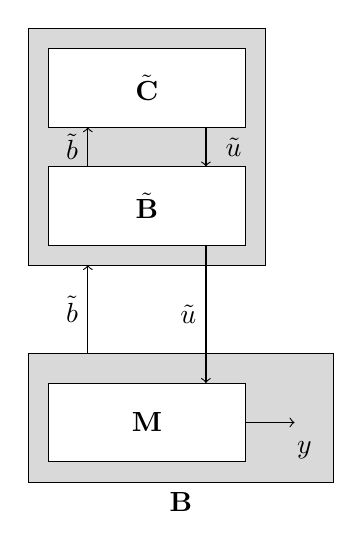
\begin{tikzpicture}

\tikzset{model/.style={
  rectangle,
  inner sep=0pt,
  text width=25mm,
  align=center,
  draw=black, fill=white,
  minimum height = 10mm
  }}
  
  \node[model] (C) at (0,2.25) {$\tilde{ \mathbf{ C}}$}; 
\node[model] (Bhat) at (0,.75) {$\tilde{ \mathbf{ B}}$}; 

%\node[label=below:$u$](bl) at (-2,.75) {};
%\node[label=below:$x$](br) at (2,.75) {};
\node(be) at (.75,1.25) {};
\node(bw) at (-.75,1.25) {};

\path[draw,<-] (be.center) -- node[label=right:$\tilde u$]{} (.75,1.75);
\path[draw,->] (bw.center) -- node[left] {$\tilde b$} (-.75,1.75);
%\path[draw,<-] (bl.center)--(Bhat);
%\path[draw,<-] (Bhat)--(br);
\node[model, fill=white](m) at (0,-2) {$\M$};
\node[](ml) at (-.75,-1.5) {};
\node[label=below:$y$](mr) at (2,-2) {};
\path[draw,->] (-.75,-1.125) -- node[left] {$\tilde b$}(-.75,0);
\path[draw,<-] (.75,-1.5) -- node[left] {$\tilde u$}(.75,.25);
\path[draw,->] (m)--(mr);
\begin{scope}[on background layer]
\node[model, fit=(ml) (mr) (m),inner sep=2.5mm,label=below:$\mathbf B$, fill=gray!30](B) {};
\node[model, fit=(C) (Bhat),inner sep=2.5mm, fill=gray!30](B) {};
\end{scope}			
\end{tikzpicture}

\caption{Control synthesis}
\end{figure}




\begin{figure}[htp]
	\centering

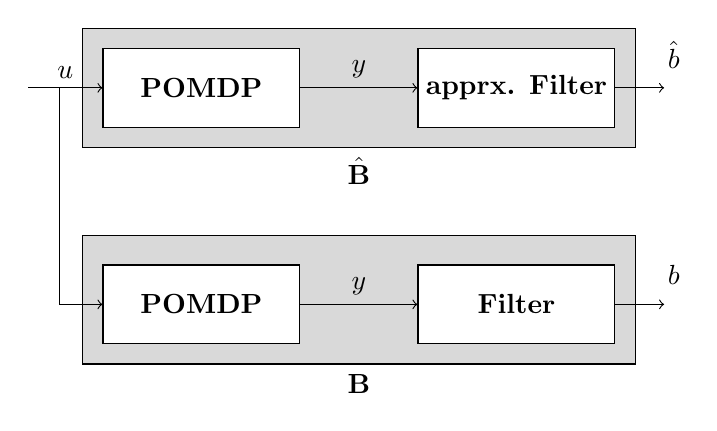
\begin{tikzpicture}

\tikzset{model/.style={
  rectangle,
  inner sep=0pt,
  text width=25mm,
  align=center,
  draw=black, fill=white,
  minimum height = 10mm
  }}
  
  \node[model] (filthat) at (4,0.75) {\textbf{apprx.  Filter}}; 
\node[model] (POMDP) at (0,.75) {\textbf{POMDP}}; 

%\node[label=below:$u$](bl) at (-2,.75) {};
%\node[label=below:$x$](br) at (2,.75) {};
\node(be) at (.75,1.25) {};
\node(bw) at (-.75,1.25) {};

%\path[draw,<-] (be.center) -- node[label=right:$\tilde u$]{} (.75,1.75);
\path[draw,->] (POMDP) -- node[above] {$y$} (filthat);
%\path[draw,<-] (bl.center)--(Bhat);
%\path[draw,<-] (Bhat)--(br);
\node[model, fill=white](m) at (0,-2) {\textbf{POMDP}};
\node[model, fill=white](filt) at (4,-2) {\textbf{Filter}};

\node[](ml) at (-.75,-1.5) {};
\node[label=above:$b$](mr) at (6,-2) {};
\node[label=above:$\hat b$](filthatr) at (6,.75) {};
\path[draw,->] (-2.2,.75) -- node[above] {$ u$}(POMDP);
\path[draw,->] (-1.8,.75) |-  (m);
\path[draw,->] (filt)--(mr);
\path[draw,->] (filthat)--(filthatr);
\path[draw,->] (m)-- node[above] {$y$}(filt);
\begin{scope}[on background layer]
\node[model, fit=(ml) (filt) (m),inner sep=2.5mm,label=below:$\mathbf B$, fill=gray!30](B) {};
\node[model, fit=(filthat) (POMDP),inner sep=2.5mm,label=below:$\hat{\mathbf{B}}$, fill=gray!30](B) {};
\end{scope}			
\end{tikzpicture}

\caption{Control synthesis}
\end{figure}





\section{Case studies}
 We detail two cases. In the first, we give a standard Gaussian LTL model and we show that one can use a constant estimator even when the noise is not constant.
 
\subsection{Flying in the wind: LTI Gaussian case}



\noindent\textbf{Point mass moving.}
    
Consider the linear time invariant system with Gaussian disturbance, given as 
\begin{align}\begin{aligned}
	x^m_{t+1} &= A x^m_{t}+B^mu_{t}+ F^m w_{t}\\
	y^m_{t}&=C^m x^m_{t}+D^m u_{t}+E^m v_{t}\end{aligned}
\end{align}
with matrices $A,B,C,D$ and matrices $F,E$. 
The disturbance signal $v$ is zero mean independently and identically  distributed noise, i.e, $w_k\sim \mathcal{N}(0,I)$.

 
 \noindent\textbf{Wind disturbance.}
We can model the dynamic variations of the wind as filtered noise. 
There are two commonly used models  \citep{richardson2013quantifying},  this includes
\begin{itemize}
	\item the von Karman power spectral density,
	\item the Dryden model.
\end{itemize}
 
 Though the former model matches experiment data more than the 
 Dryden model, the Dryden model can be represented by  a lower order filter.
 
Consider a filter model to be given as
\begin{align}
	\begin{aligned}
	x_{t+1}^w &= A^w x_{t}^w+ F^w e_{t},\\
	w_{t}&=C^w x_{t}^w+E^w e_{t}.
	\end{aligned}
\end{align}

\textbf{Full model \& Belief space model.}
The full model is given as follows
\begin{align} 
	\begin{bmatrix}
	x^m_{t+1}	\\x^w_{t+1}
	\end{bmatrix}
 &= \begin{bmatrix}
 	A^m 	& F^mC^w\\
 	0 & A^w
 \end{bmatrix}
\begin{bmatrix}
	x^m_{t}	\\x^w_{t}
	\end{bmatrix}+\begin{bmatrix} B^m \\ 0~ \end{bmatrix} u_{t}+  \begin{bmatrix}
	F^m E^w \\
	F^w
	\end{bmatrix}e_{t}\notag\\
	y^m_{t}&=\begin{bmatrix} C^m& 0 \end{bmatrix}\begin{bmatrix}
	x^m_{t}	\\x^w_{t}
	\end{bmatrix}+D^m u_{t}+E^m v_{t}.
\end{align}
This can be written as 
 \begin{align}  \begin{aligned}
x_{t+1}&=A x_{t} + B u_t+ Fe_t\\
y_t&=Cx_t+Du_t+Ev_t\end{aligned} \end{align}
\begin{align}& \mbox{ with }  x_t	= \begin{bmatrix}
	x^m_{t}	\\x^w_{t}
	\end{bmatrix},
A = \begin{bmatrix}
 	A^m 	& F^mC^w\\
 	0 & A^w
 \end{bmatrix}, \ 
B = \begin{bmatrix} B^m \\ 0~ \end{bmatrix}\notag \\
&F=\begin{bmatrix}
	F^m E^w \\
	F^w
	\end{bmatrix},\ 
C = \begin{bmatrix} C^m& 0 \end{bmatrix} , \ 
D= D^m, \  E = E^m.\notag
\end{align}
 
 
The belief space $\mathbb{B}$ is  a finite dimensional space and can be parameterized . For example, let $\CA{G}$ denote the Gaussian belief space
    of dimension $n$, i.e. the space of Gaussian
    probability measures over $\BB{R}^n$.
    For brevity, we identify the Gaussian measures
    with their finite parametrization, mean and
    covariance matrix.
     Thus,
    $\CA{G} =  \BB{R}^n \times  \S^n$.
    
    
 
 In the second case, we leverage the developed simulation relation for FIRM. 
 
 \red{[SEARCHING FOR A GOOD CASE! What about the rover? Or rover driving over uncertain map elements?]}



%% Bibiliography %%%%%%%%%%%%%%%%%%%%%%%%
\bibliography{AliAgha,references}

%%%%%%%%%%%%%%%%%%%%%%%%%%%%%%%%%%




\end{document}

